\documentclass[
11pt, % The default document font size, options: 10pt, 11pt, 12pt
codirector, % Uncomment to add a codirector to the title page
]{charter}

% El títulos de la memoria, se usa en la carátula y se puede usar el cualquier lugar del documento con el comando \ttitle
\titulo{Controlador de pH para cultivos hidropónicos}

% Nombre del posgrado, se usa en la carátula y se puede usar el cualquier lugar del documento con el comando \degreename
\posgrado{Carrera de Especialización en Sistemas Embebidos} 
%\posgrado{Carrera de Especialización en Internet de las Cosas} 
%\posgrado{Carrera de Especialización en Inteligencia Artificial}
%\posgrado{Maestría en Sistemas Embebidos} 
%\posgrado{Maestría en Internet de las cosas}
% IMPORTANTE: no omitir titulaciones ni tildación en los nombres, también se recomienda escribir los nombres completos (tal cual los tienen en su documento)
% Tu nombre, se puede usar el cualquier lugar del documento con el comando \authorname
\autor{Ing. Iván Podoroska}

% El nombre del director y co-director, se puede usar el cualquier lugar del documento con el comando \supname y \cosupname y \pertesupname y \pertecosupname
\director{Ing. Juan Pepito}
\pertenenciaDirector{pertenencia} 
\codirector{} % para que aparezca en la portada se debe descomentar la opción codirector en los parámetros de documentclass
\pertenenciaCoDirector{}

% Nombre del cliente, quien va a aprobar los resultados del proyecto, se puede usar con el comando \clientename y \empclientename
\cliente{Francisco Yuvone}
\empresaCliente{Cannfeel SA}
 
\fechaINICIO{29 de abril de 2024}		%Fecha de inicio de la cursada de GdP \fechaInicioName
\fechaFINALPlan{11 de junio de 2024} 	%Fecha de final de cursada de GdP
\fechaFINALTrabajo{14 de noviembre de 2024}	%Fecha de defensa pública del trabajo final


\begin{document}

\maketitle
\thispagestyle{empty}
\pagebreak


\thispagestyle{empty}
{\setlength{\parskip}{0pt}
\tableofcontents{}
}
\pagebreak

\section*{Registros de cambios}
\label{sec:registro}


\begin{table}[ht]
\label{tab:registro}
\centering
\begin{tabularx}{\linewidth}{@{}|c|X|c|@{}}
\hline
\rowcolor[HTML]{C0C0C0} 
Revisión & \multicolumn{1}{c|}{\cellcolor[HTML]{C0C0C0}Detalles de los cambios realizados} & Fecha      \\ \hline
0      & Creación del documento                                 &\fechaInicioName \\ \hline
1      & Se completa hasta el punto 5 inclusive                 & {7} de {mayo} de 2024 \\ \hline
2      & Se completa hasta el punto 9 inclusive					& {14} de {mayo} de 2024 \\ \hline
3      & Se completa hasta el punto 12 inclusive                & {21} de {mayo} de 2024 \\ \hline
4      & Se completa el plan	                                & {28} de {mayo} de 2024 \\ \hline
%		  Se puede agregar algo más \newline
%		  En distintas líneas \newline
%		  Así                                                    & {día} de {mes} de 202X \\ \hline

% Si hay más correcciones pasada la versión 4 también se deben especificar acá

\end{tabularx}
\end{table}

\pagebreak



\section*{Acta de constitución del proyecto}
\label{sec:acta}

\begin{flushright}
Buenos Aires, \fechaInicioName
\end{flushright}

\vspace{2cm}

Por medio de la presente se acuerda con el Ing. \authorname\hspace{1px} que su Trabajo Final de la \degreename\hspace{1px} se titulará ``\ttitle'' y consistirá en la implementación de un prototipo de un sistema de control de pH para cultivos hidropónicos. El trabajo tendrá un presupuesto preliminar estimado de 648 horas y un costo de \$13111000, con fecha de inicio el \fechaInicioName\hspace{1px} y fecha de presentación pública el \fechaFinalName.

Se adjunta a esta acta la planificación inicial.

\vfill

% Esta parte se construye sola con la información que hayan cargado en el preámbulo del documento y no debe modificarla
\begin{table}[ht]
\centering
\begin{tabular}{ccc}
\begin{tabular}[c]{@{}c@{}}Dr. Ing. Ariel Lutenberg \\ Director posgrado FIUBA\end{tabular} & \hspace{2cm} & \begin{tabular}[c]{@{}c@{}}\clientename \\ \empclientename \end{tabular} \vspace{2.5cm} \\ 
\multicolumn{3}{c}{\begin{tabular}[c]{@{}c@{}} \supname \\ Director del Trabajo Final\end{tabular}} \vspace{2.5cm} \\
\end{tabular}
\end{table}




\section{1. Descripción técnica-conceptual del proyecto a realizar}
\label{sec:descripcion}

La agricultura hidropónica es un método utilizado para cultivar plantas sin tierra, usando una solución rica en nutrientes. Mediante el contacto directo de las raíces con la solución nutritiva se logra un suministro constante y eficiente de macronutrientes y micronutrientes esenciales. Para su absorción, intervienen procesos de transporte activo y ósmosis, que requieren un pH controlado para garantizar el transporte de los nutrientes hacia la planta.

La empresa Cannfeel incorpora equipos para la medición y control de cultivos de precisión mediante Internet de las Cosas (IOT, por sus siglas en inglés). El objetivo de este proyecto es sumar un producto más al ecosistema, que sea capaz de regular y controlar el pH de soluciones nutritivas. Deberá poder integrarse a los equipos existentes y funcionar de manera autónoma.

El proyecto permitirá abstraer al cultivador de la tarea manual de la regulación del pH de la solución nutritiva. Al estar incluida en el ecosistema de la empresa, el usuario podrá tener acceso en tiempo real al estado de la solución nutritiva a través de una aplicación web ya implementada.

El sistema deberá ser capaz de medir el pH y la temperatura de una solución nutritiva. Contará con un \textit{encoder} rotativo con botón y una pantalla, donde el usuario podrá ingresar el valor de pH que desee para la solución. El sistema tendrá que ser capaz de controlar el pH, utilizando una solución \textit{buffer}. Para llevar a cabo la inyección de la sustancia reguladora, se contará con una bomba peristáltica como se observa en la figura \ref{fig:diagBloq}.

El reto del presente proyecto es poder implementar tanto el hardware como el firmware asociado para alcanzar la solución propuesta en el tiempo estimado.

En la figura \ref{fig:diagBloq} se representa el diagrama en bloques del sistema.

\begin{figure}[htpb]
\centering 
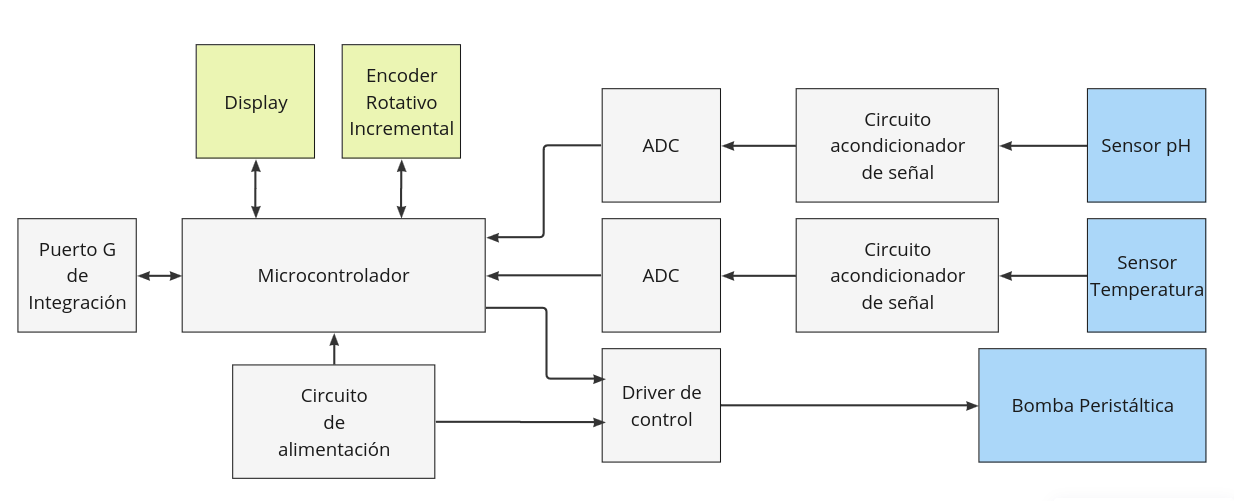
\includegraphics[width=.85\textwidth]{./Figuras/diagBloq.png}
\caption{Diagrama en bloques del sistema.}
\label{fig:diagBloq}
\end{figure}

En la figura \ref{fig:diagCtrl} se representa el diagrama en bloque del esquema de control a implementar.

\begin{figure}[htpb]
\centering
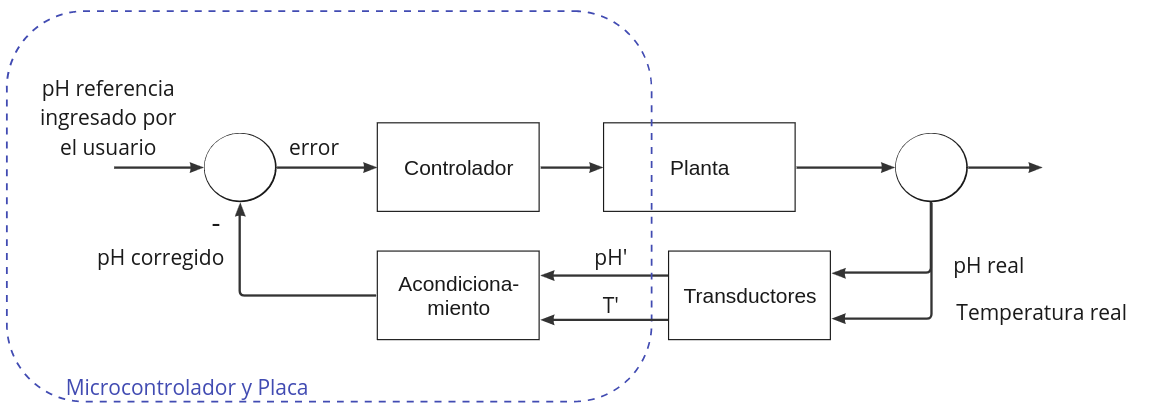
\includegraphics[width=.85\textwidth]{./Figuras/diagCtrl.png}
\caption{Diagrama de control del sistema.}
\label{fig:diagCtrl}
\end{figure}


\section{2. Identificación y análisis de los interesados}
\label{sec:interesados}

\begin{table}[ht]
%\caption{Identificación de los interesados}
%\label{tab:interesados}
\begin{tabularx}{\linewidth}{@{}|l|X|X|l|@{}}
\hline
\rowcolor[HTML]{C0C0C0} 
Rol           & Nombre y Apellido & Organización 	& Puesto 	\\ \hline
%Auspiciante   &                   &              	&        	\\ \hline
Cliente       & \clientename      &\empclientename	& CTO      	\\ \hline
%Impulsor      &                   &              	&        	\\ \hline
Responsable   & \authorname       & FIUBA        	& Alumno 	\\ \hline
%Colaboradores &                   &              	&        	\\ \hline
Orientador    & \supname	      & \pertesupname 	& Director del Trabajo Final \\ \hline
%Equipo        & miembro1 \newline 
%				miembro2          &              	&        	\\ \hline
%Opositores    &                   &              	&        	\\ \hline
%Usuario final &                   &              	&        	\\ \hline
\end{tabularx}
\end{table}

\section{3. Propósito del proyecto}
\label{sec:proposito}

Desarrollar un prototipo funcional capaz de medir y controlar en línea el pH de una solución nutritiva para cultivos hidropónicos. Se busca que el cultivador no deba realizar de manera manual esta tarea.

\section{4. Alcance del proyecto}
\label{sec:alcance}

El presente proyecto incluye:
\begin{itemize}
	\item Diseño e implementación de un prototipo.
		\begin{itemize}
		\item Diseño de hardware.
		\item Diseño de firmware.
		\end{itemize}
	\item Elección del display para la interfaz.
	\item Elección del \textit{encoder} rotativo.
	\item Elección del sensor de pH.
	\item Elección del método de sensado de temperatura.
		\begin{itemize}
		\item Elección del sensor de temperatura.
		\end{itemize}
	\item Elección de la bomba peristáltica.
	\item Ensayos de funcionamiento en campo.
\end{itemize}

El presente proyecto no incluye:
\begin{itemize}
	\item Diseño y fabricación de la carcaza del dispositivo.
	\item Modificaciones en la aplicación web existente.
	\item Manual de usuario.
	\item Manual de instalación.
\end{itemize}


\section{5. Supuestos del proyecto}
\label{sec:supuestos}


\begin{itemize}
	\item Se tendrá a disposición los equipos de la empresa Cannfeel SA cuando sean requeridos.
	\item Se utilizarán herramientas que no requieran licencia.
	\item Todos los componentes estarán disponibles para su compra.
	\item Será posible desarrollar los PCBs del prototipo de prueba.
	\item Los tiempos de importación y de fabricación estarán dentro de lo planeado.
	\item No habrá problemas para la importación de lo requerido.
	\item El presupuesto no superará en gran medida a lo estimado.
\end{itemize}


\section{6. Requerimientos}
\label{sec:requerimientos}

\begin{enumerate}
	\item Requerimientos técnicos
		\begin{enumerate}
			\item El sistema se deberá alimentar con una fuente de alimentación externa.
			\item El hardware deberá tener un driver para manejar una bomba peristáltica.
			\item El hardware deberá contar con un conector para una sonda de pH.
			\item El hardware deberá contar con un conector para una sonda de temperatura.
			\item El hardware deberá acondicionar la señal de la sonda de pH.
			\item El hardware deberá acondicionar la señal de la sonda de temperatura.
			\item El sistema deberá encender y apagar una bomba de recirculación opcional.
		\end{enumerate}
		
	\item Requerimientos funcionales
		\begin{enumerate}
			\item El sistema deberá compensar la medición de pH con la temperatura de la solución.
			\item El sistema deberá reconocer una falla por falta de solución \textit{buffer}.
			\item El sistema deberá reconocer si no puede controlar el pH de la solución nutritiva.
			\item El sistema deberá tener un modo de control donde intente corregir el pH de la solución constantemente.
			\item El sistema deberá contar con un modo de solo lectura que se limite a mostrar en la pantalla los valores obtenidos de los sensores.
			\item El sistema deberá contar con un modo de configuración donde se podrán calibrar los sensores y configurar el valor deseado de pH para el control.
		\end{enumerate}
		
	\item Requerimientos de interoperabilidad
		\begin{enumerate}
			\item El controlador se deberá integrar al ecosistema de dispositivos de la empresa Cannfeel mediante un protocolo propietario.
		\end{enumerate}	
		
	\item Requerimientos de la interfaz
		\begin{enumerate}
			\item El hardware deberá contar con una pantalla no táctil.
			\item El hardware deberá contar con un \textit{encoder} rotativo incremental con botón.
			\item El sistema permitirá configurar los parámetros del controlador desde la interfaz local.
			\item El usuario deberá poder calibrar la sonda de pH en tres puntos desde la interfaz local.
			\item El usuario deberá poder calibrar la sonda de temperatura desde la interfaz local.
		\end{enumerate}
		
	\item Requerimientos de pruebas
		\begin{enumerate}
			\item El sistema no deberá funcionar en modo de regulación si detecta la falta de solución \textit{buffer}.
		\end{enumerate}
		
	\item Requerimientos de documentación
		\begin{enumerate}
			\item Se confeccionarán informes de avance dirigidos al cliente y al director con la finalidad de controlar el avance del proyecto.
			\item Se confeccionará una memoria técnica al finalizar el proyecto.
		\end{enumerate}
\end{enumerate}

\section{7. Historias de usuarios (\textit{Product backlog})}
\label{sec:backlog}

En esta sección se mostrarán las historias de usuarios según los roles de: cliente, usuario final y desarrollador. Se valoraron de acuerdo a un sistema de \textit{story points} basado en la estimación de tres categorías:

\begin{itemize}
	\item Complejidad del trabajo (C):
	\begin{itemize}
		\item Bajo: 1
		\item Medio: 5
		\item Alto: 13		
	\end{itemize}
	\item Dificultad del trabajo (D):
	\begin{itemize}
		\item Bajo: 1
		\item Medio: 3
		\item Alto: 5		
	\end{itemize}
	\item Riesgo del trabajo (R):
	\begin{itemize}
		\item Bajo: 1
		\item Medio: 3
		\item Alto: 5		
	\end{itemize}
\end{itemize}

Para obtener la estimación final, se sumaron los valores asignados a cada aspecto y se aproximaron
al siguiente número de la serie de Fibonacci. Por ejemplo, si la complejidad del trabajo es media (5), la dificultad es alta (5) y la incertidumbre es media (3), las suma de los \textit{story points} es 13 y se aproxima al siguiente número de Fibonacci, que es 21. La valoración final será 21.

\begin{enumerate}
	\item Como cliente, quiero que el sistema sea capaz de comunicarse con otros dispositivos del ecosistema de la empresa para que se integren y mejoren la solución ofrecida. 
	\begin{itemize}
		\item \textit{Story points}: 8 (C:1, D:5, R:1).	
	\end{itemize}
	
	\item Como usuario final, quiero modificar los parámetros de medición del sensor de pH con el objetivo de calibrarlo.
	\begin{itemize}
		\item \textit{Story points}: 3 (C:1, D:1, R:1).	
	\end{itemize}
	
	\item Como usuario final, quiero poder configurar el valor de pH a controlar de manera local para no depender de la conexión a una plataforma. 
	\begin{itemize}
		\item \textit{Story points}: 21 (C:13, D:3, R:3).	
	\end{itemize}
	
	\item Como desarrollador, quiero implementar un controlador de pH preciso y de bajo costo para poder controlar la absorción de nutrientes de las plantas en cultivos hidropónicos.
	\begin{itemize}
		\item \textit{Story points}: 21 (C:13, D:5, R:3).	
	\end{itemize}
\end{enumerate}

\section{8. Entregables principales del proyecto}
\label{sec:entregables}

Los entregables de proyecto son:

\begin{itemize}
	\item Prototipo funcional.
	\item Archivos para la producción del PCB.
	\item Diagrama de circuitos esquemáticos.
	\item Lista de materiales (BOM, por sus siglas en inglés).
	\item Código fuente del firmware.
	\item Informes de avance.
	\item Memoria del trabajo final.
\end{itemize}

\section{9. Desglose del trabajo en tareas}
\label{sec:wbs}

\begin{enumerate}
\item Investigación y documentación (92 h)
	\begin{enumerate}
	\item Investigar sobre el estado del arte (8 h).
	\item Armar el plan de proyecto (32 h).
	\item Investigación y elección de sensor de pH (16 h).
	\item Investigación y elección de sensor de temperatura (16 h).
	\item Investigación y elección de pantalla (12 h).
	\item Investigación y elección de \textit{encoder} rotativo incremental (8 h).
	\end{enumerate}
	
\item Diseño general (36 h)
	\begin{enumerate}
	\item Diseño de diagrama de módulos (8 h).
	\item Diseño de diagrama de conexiones (8 h).
	\item Elección de la fuente de alimentación externa (4 h).
	\item Diseño de las interfaces de la pantalla (16 h).
	\end{enumerate}
	
\item Desarrollo del hardware (132 h)
	\begin{enumerate}
	\item Elección de conectores y componentes de potencia (24 h).
	\item Selección de componentes varios (8 h).
	\item Diseño de diagramas esquemáticos (40 h).
	\item Diseño del PCB y de los archivos de fabricación (40 h).
	\item Armado del prototipo (20 h).
	\end{enumerate}
	
\item Desarrollo del firmware (244 h)
	\begin{enumerate}
	\item Elección de la arquitectura (12 h).
	\item Diseño en papel de los módulos a implementar (12 h).
	\item Diseño de las máquinas de estados (40 h).
	\item Diseño de pruebas (40 h).
	\item Programación de firmware (100 h).
	\item Verificación y validación (40 h).
	\end{enumerate}
	
\item Pruebas y calibración (52 h)
	\begin{enumerate}
	\item Prueba del prototipo en modo de funcionamiento normal (20 h).
	\item Prueba del prototipo en modo de funcionamiento en falla (16 h).
	\item Ajustes finales y puesta a punto (16 h).
	\end{enumerate}
	
\item Presentación final (92 h)
	\begin{enumerate}
	\item Redacción del informe de avances (12 h)
	\item Redacción de la memoria técnica (60 h).
	\item Presentación final (20 h).
	\end{enumerate}
\end{enumerate}

Cantidad total de horas: 648 h.

\section{10. Diagrama de Activity On Node}
\label{sec:AoN}

\begin{figure}[htpb]
\centering 
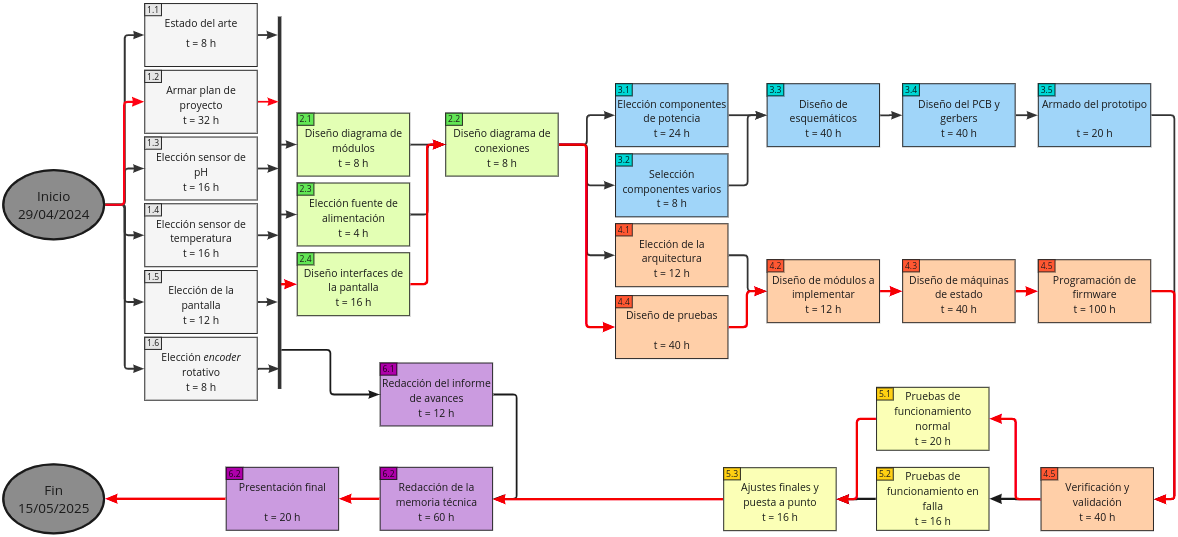
\includegraphics[width=1\textwidth]{./Figuras/AoN-1.png}
\caption{Diagrama de \textit{Activity on Node}.}
\label{fig:AoN}
\end{figure}

En rojo se marca el camino crítico.

\section{11. Diagrama de Gantt}
\label{sec:gantt}

En la figura \ref{fig:gantt-1} y \ref{fig:gantt-2} se muestran el diagrama de Gantt correspondiente a las tareas detalladas en la figura \ref{fig:tasks}. Se toma un calendario de 5 días laborales por semana y se estima un trabajo de 20 horas semanales dividido en 4 horas diarias. Cada 'd' del diagrama representa 4 horas.

\begin{figure}[htpb]
\centering 
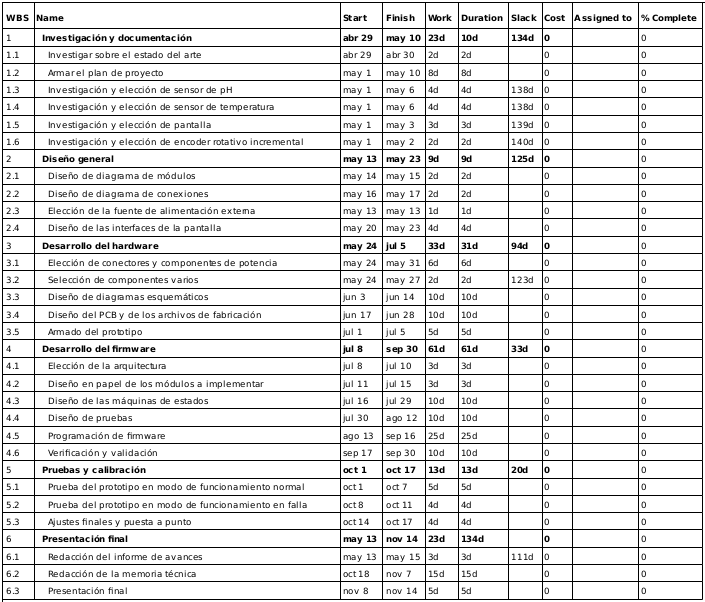
\includegraphics[width=1\textwidth]{./Figuras/tasks.png}
\caption{Tabla de diagrama de Gantt.}
\label{fig:tasks}
\end{figure}

\begin{figure}[htpb]
\centering 
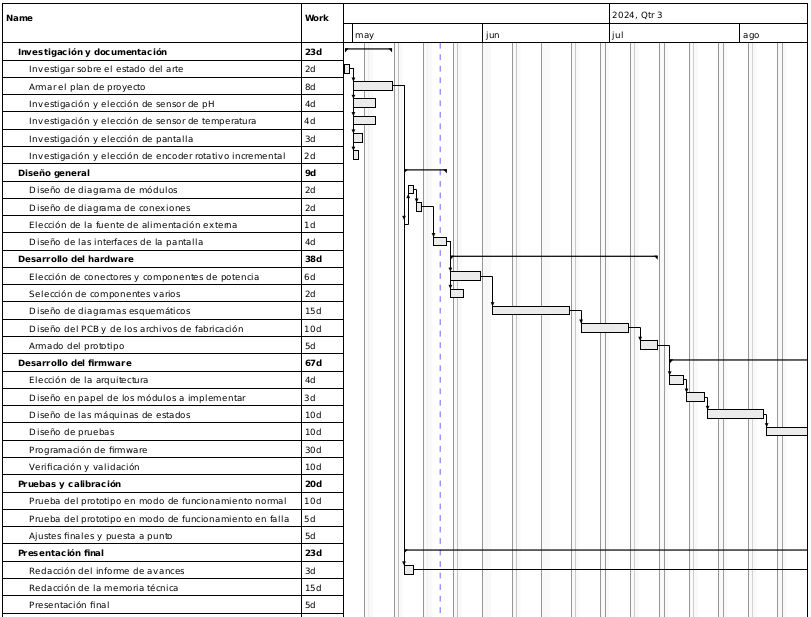
\includegraphics[width=1\textwidth]{./Figuras/gantt-1.png}
\caption{Diagrama de Gantt 1}
\label{fig:gantt-1}
\end{figure}

\begin{figure}[htpb]
\centering 
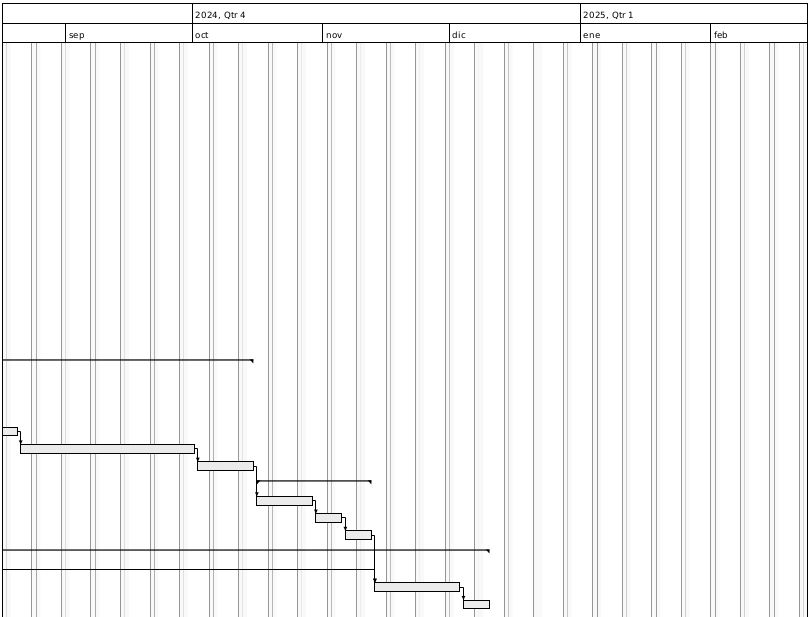
\includegraphics[width=1\textwidth]{./Figuras/gantt-2.png}
\caption{Diagrama de Gantt 2}
\label{fig:gantt-2}
\end{figure}

\section{12. Presupuesto detallado del proyecto}
\label{sec:presupuesto}

Para la siguiente estimación de costos se toma 1 USD = 1000 ARS como tasa de cambio.

\begin{table}[htpb]
\centering
\begin{tabularx}{\linewidth}{@{}|X|c|r|r|@{}}
\hline
\rowcolor[HTML]{C0C0C0} 
\multicolumn{4}{|c|}{\cellcolor[HTML]{C0C0C0}COSTOS DIRECTOS} \\ \hline
\rowcolor[HTML]{C0C0C0} 
Descripción &
  \multicolumn{1}{c|}{\cellcolor[HTML]{C0C0C0}Cantidad} &
  \multicolumn{1}{c|}{\cellcolor[HTML]{C0C0C0}Valor unitario} &
  \multicolumn{1}{c|}{\cellcolor[HTML]{C0C0C0}Valor total} \\ \hline
 
 Salario ingeniero &
  \multicolumn{1}{c|}{ 648 } &
  \multicolumn{1}{c|}{ USD 15 } &
  \multicolumn{1}{c|}{ USD 9720 } \\ \hline
  
 Punta de prueba de pH &
  \multicolumn{1}{c|}{ 1 } &
  \multicolumn{1}{c|}{ USD 100 } &
  \multicolumn{1}{c|}{ USD 100 } \\ \hline
  
 Soluciones \textit{buffers} de calibración &
  \multicolumn{1}{c|}{ 3 } &
  \multicolumn{1}{c|}{ USD 10 } &
  \multicolumn{1}{c|}{ USD 30 } \\ \hline
  
 Bomba peristáltica &
  \multicolumn{1}{c|}{ 1 } &
  \multicolumn{1}{c|}{ USD 100 } &
  \multicolumn{1}{c|}{ USD 100 } \\ \hline
  
 Manguera de silicona &
  \multicolumn{1}{c|}{ 1 } &
  \multicolumn{1}{c|}{ USD 20 } &
  \multicolumn{1}{c|}{ USD 20 } \\ \hline

 Sensor de temperatura &
  \multicolumn{1}{c|}{ 1 } &
  \multicolumn{1}{c|}{ USD 50 } &
  \multicolumn{1}{c|}{ USD 50 } \\ \hline
  
 Encoder rotativo con botón &
  \multicolumn{1}{c|}{ 1 } &
  \multicolumn{1}{c|}{ USD 5 } &
  \multicolumn{1}{c|}{ USD 5 } \\ \hline
  
 Fuente de alimentación &
  \multicolumn{1}{c|}{ 1 } &
  \multicolumn{1}{c|}{ USD 10 } &
  \multicolumn{1}{c|}{ USD 10 } \\ \hline   

 Componentes varios para el prototipo &
  \multicolumn{1}{c|}{ 1 } &
  \multicolumn{1}{c|}{ USD 50 } &
  \multicolumn{1}{c|}{ USD 50 } \\ \hline  
  
\multicolumn{3}{|c|}{SUBTOTAL} &
  \multicolumn{1}{c|}{ USD 10085 } \\ \hline
  
\rowcolor[HTML]{C0C0C0}
\multicolumn{4}{|c|}{\cellcolor[HTML]{C0C0C0}COSTOS INDIRECTOS} \\ \hline
\rowcolor[HTML]{C0C0C0} 
Descripción &
  \multicolumn{1}{c|}{\cellcolor[HTML]{C0C0C0}Cantidad} &
  \multicolumn{1}{c|}{\cellcolor[HTML]{C0C0C0}Valor unitario} &
  \multicolumn{1}{c|}{\cellcolor[HTML]{C0C0C0}Valor total} \\ \hline
 
\multicolumn{1}{|l|}{30\% del costo directo} &
   \multicolumn{1}{c|}{ 1 } &
   \multicolumn{1}{c|}{ USD 3026 } &
   \multicolumn{1}{c|}{ USD 3026 }\\ \hline
   
\multicolumn{3}{|c|}{SUBTOTAL} &
  \multicolumn{1}{c|}{ USD 3026 } \\ \hline
\rowcolor[HTML]{C0C0C0}
\multicolumn{3}{|c|}{TOTAL} &
   USD 13111\\ \hline
\end{tabularx}%
\end{table}


\section{13. Gestión de riesgos}
\label{sec:riesgos}

a) Identificación de los riesgos y estimación de sus consecuencias:

Riesgo 1: Problemas de compatibilidad o limitaciones en las herramientas sin licencia seleccionadas para llevar a cabo el proyecto.
\begin{itemize}
	\item Severidad (6): Darse cuenta en una etapa avanzada del proyecto de un problema de este tipo, puede representar una importante pérdida tiempo.
	\item Probabilidad de ocurrencia (4):  Las herramientas sin licencia son ampliamente utilizadas, pero las limitaciones no siempre son evidentes.
\end{itemize}

Riesgo 2: Que los componentes requeridos para el prototipo no estén disponibles para la compra.
\begin{itemize}
	\item Severidad (8): La falta de componentes puede detener el desarrollo y pruebas del hardware retrasando el proyecto.
	\item Probabilidad de ocurrencia (7): Hay poca disponibilidad de componentes específicos, o de precisión, en el mercado local.
\end{itemize}

Riesgo 3: Falta de disponibilidad de equipos de Cannfeel SA requeridos para las pruebas.
\begin{itemize}
	\item Severidad (8): Causaría retrasos en las pruebas y el desarrollo del proyecto.
	\item Probabilidad de ocurrencia (4): Existe \textit{stock} de los dispositivos requeridos. 
\end{itemize}

Riesgo 4:  Características del hardware seleccionado insuficientes para satisfacer las necesidades
del sistema.
\begin{itemize}
	\item Severidad (8): Podría causar un mal funcionamiento del equipo en etapas avanzadas del proyecto.
	\item Probabilidad de ocurrencia (3): El hardware será verificado y validado por el director. 
\end{itemize}

Riesgo 5:  Informe de avances inadecuado.
\begin{itemize}
	\item Severidad (7): La falta de transparencia y comunicación puede conducir a tomas de decisiones erroneas.
	\item Probabilidad de ocurrencia (2): Las reuniones mensuales y continua comunicación con el director disminuyen la ocurrencia de este riesgo. 
\end{itemize}


b) Tabla de gestión de riesgos:      (El RPN se calcula como RPN=SxO)

\begin{table}[htpb]
\centering
\begin{tabularx}{\linewidth}{@{}|X|c|c|c|c|c|c|@{}}
\hline
\rowcolor[HTML]{C0C0C0} 
Riesgo & S & O & RPN & S* & O* & RPN* \\ \hline
   1   & 6 & 4 &  24 &    &    &      \\ \hline
   2   & 8 & 7 &  56 & 5  & 4  & 20   \\ \hline
   3   & 8 & 4 &  32 & 8  & 2  & 20   \\ \hline
   4   & 8 & 3 &  24 &    &    &      \\ \hline
   5   & 7 & 2 &  14 &    &    &      \\ \hline
\end{tabularx}%
\end{table}

Criterio adoptado: 

Se tomarán medidas de mitigación en los riesgos cuyos números de RPN sean mayores a 30.

Nota: los valores marcados con (*) en la tabla corresponden luego de haber aplicado la mitigación.

c) Plan de mitigación de los riesgos que originalmente excedían el RPN máximo establecido:

Acción de mitigación del riesgo 2:	Identificar proveedores en el país de componentes electrónicos y consultar disponibilidad de componentes. Diseñar en función de la disponibilidad local y capacidad de reemplazo.

\begin{itemize}
	\item Severidad (5): Mediante un diseño basado en la disponibilidad, el riesgo disminuye.
	\item Probabilidad de ocurrencia (4): La aparición de posibles reemplazos disminuye la ocurrencia inicial.
\end{itemize}

Acción de mitigación del riesgo 3:	Reservar con antelación los equipos que se necesitarán para hacer
las pruebas requeridas.
\begin{itemize}
	\item Severidad (8): El riesgo seguirá existiendo.
	\item Probabilidad de ocurrencia (2): La ocurrencia disminuye debido a las acciones de previsión.
\end{itemize}


\section{14. Gestión de la calidad}
\label{sec:calidad}

\begin{itemize} 

\item Requerimiento 1.2: El hardware deberá tener un driver para manejar una bomba peristáltica.

\begin{itemize}
	\item Verificación: Asegurarse que el diseño del hardware incluye un driver adecuado para controlar una bomba peristáltica. Verificar que los esquemáticos y las especificaciones del driver cumplen con los requisitos de la bomba peristáltica.
	\item Validación: Activar y controlar la bomba peristáltica utilizando el driver y verificar el correcto funcionamiento.
\end{itemize}

\item Requerimiento 1.7: El sistema deberá encender y apagar una bomba de recirculación opcional.

\begin{itemize}
	\item Verificación: Asegurarse que el diseño de hardware y de firmware incluyen la capacidad de controlar una bomba de recirculación opcional.
	\item Validación: Activar el control de la bomba y verificar que el sistema la puede encender y apagar.
\end{itemize}

\item Requerimiento 2.1: El sistema deberá compensar la medición de pH con la temperatura de la solución.

\begin{itemize}
	\item Verificación: Se analizarán distintos métodos de medición con sus compensaciones.
	\item Validación: Realizar mediciones de pH a diferentes temperaturas y validar que el sistema compensa adecuadamente las lecturas.
\end{itemize}

\item Requerimiento 2.2: El sistema deberá reconocer una falla por falta de solución \textit{buffer}.

\begin{itemize}
	\item Verificación: Asegurarse que el diseño de hardware y de firmware incluye mecanismos para detectar la presencia o ausencia de la solución \textit{buffer}.
	\item Validación: Simular la condición de falta de solución \textit{buffer} y validar que el sistema reconoce la falla y notifica adecuadamente.
\end{itemize}

\item Requerimiento 2.3: El sistema deberá reconocer si no puede controlar el pH de la solución nutritiva.

\begin{itemize}
	\item Verificación: Verificar que el algoritmo de detección de fallos en el control del pH está implementado correctamente en el código.
	\item Validación: Simular condiciones en las que el sistema no puede controlar el pH y validar que la falla se reconoce y notifica adecuadamente.
\end{itemize}

\item Requerimiento 2.4: El sistema deberá tener un modo de control donde intente corregir el pH de la solución constantemente.

\begin{itemize}
	\item Verificación: Verificar que el algoritmo de control de pH está implementado correctamente en el código.
	\item Validación: Activar el modo de control de pH y verificar que el sistema lo corrige continuamente.
\end{itemize}

\item Requerimiento 2.5: El sistema deberá contar con un modo de solo lectura que se limite a mostrar en la pantalla los valores obtenidos de los sensores.

\begin{itemize}
	\item Verificación: Verificar que la interfaz de usuario y el firmware están implementados para soportar este modo.
	\item Validación: Monitorear el comportamiento del sistema durante un período prolongado para asegurar que mantiene la funcionalidad de solo lectura sin fallos.
\end{itemize}

\item Requerimiento 2.6: El sistema deberá contar con un modo de configuración donde se podrán calibrar los sensores y configurar el valor deseado de pH para el control.

\begin{itemize}
	\item Verificación: Corroborar que la interfaz de usuario y el firmware están implementados para soportar la calibración de los sensores y la configuración del valor de pH.
	\item Validación: Verificar que los sensores pueden ser calibrados correctamente. Configurar el valor deseado de pH y corroborar que el sistema guarda y utiliza este valor correctamente.
\end{itemize}

\item Requerimiento 3.1: El controlador se deberá integrar al ecosistema de dispositivos de la empresa Cannfeel mediante un protocolo propietario.

\begin{itemize}
	\item Verificación: Lectura de los documentos internos de funcionamiento del protocolo. Corroboración de la implementacion en el firmware.
	\item Validación: Demostración de funcionamiento dentro del ecosistema de la empresa.
\end{itemize}

\item Requerimiento 4.1: El hardware deberá contar con una pantalla no táctil.

\begin{itemize}
	\item Verificación: Asegurarse que el diseño del hardware incluye una pantalla no táctil que cumple con los requisitos del proyecto.
	\item Validación: Verificar que la pantalla muestra la información esperada de manera clara y precisa. Monitorear el comportamiento durante un período prolongado para asegurar un funcionamiento confiable.
\end{itemize}

\end{itemize}

\section{15. Procesos de cierre}    
\label{sec:cierre}

Se establecen las siguientes actividades de finalización de proyecto:

\begin{itemize}
	
	\item Analizar si se respetó el Plan de Proyecto original teniendo en cuenta las fechas y duración de las tareas. Se hará lo mismo con los costos y riesgos previstos desde el comienzo.
	
	Para llevar a cabo esta acividad, se confeccionará una hoja de cálculo comparativa y se contrastará lo estimado con lo real.
	\begin{itemize}
		\item Responsable: Ing. Iván Podoroska.
	\end{itemize}
	
	\item Identificación de las técnicas y procedimientos útiles e inútiles que se utilizaron, y los
problemas que surgieron y cómo se solucionaron.
	\begin{itemize}
		\item Responsable: Ing. Iván Podoroska.
	\end{itemize}
	
	\item Archivado de toda la documentación requerida y generada para la realización del proyecto.
	\begin{itemize}
		\item Responsable: Ing. Iván Podoroska.
	\end{itemize}
	
	\item Acto de cierre y finalización de proyecto. Se agradecerá a todas las partes involucradas.
	\begin{itemize}
		\item Responsable: Sr. Francisco Yuvone.
	\end{itemize}
	
\end{itemize}

\end{document}